\section{Power Management Dynamique}

\begin{frame}
	\frametitle{Power Management Dynamique}
	\center{\Large{Minimiser la consommation d'un système actif}}
	\begin{block}{Compromis}
	\begin{itemize}
		\item Ressources utilisées
		\item Ressources nécessaires
		\item Latences acceptables
		\item Consommation actuelle
		\item Température actuelle
	\end{itemize}
	\end{block}
\end{frame}

\begin{frame}[fragile]
	\frametitle{PM pour les périphériques}
	\begin{block}{PM core}
		\begin{itemize}
			\item API pour drivers
			\item Interface sysfs
			\item PM dynamique
			\item Modes d'endormissement
		\end{itemize}
	\end{block}
	\textbf{Documentation} : \texttt{Documentation/power}

	\textbf{Headers} : \texttt{include/linux/pm.h}

	\textbf{Implémentation} : \texttt{kernel/power/}
\end{frame}
\begin{frame}[fragile]
	\frametitle{runtime\_pm}
	\begin{block}{Etats}
		\begin{itemize}
			\item \texttt{active} : Est capable d'I/O
			\item \texttt{suspended} : Pas d'I/O
		\end{itemize}
	\end{block}
	\begin{minipage}[t]{0.45\linewidth}
		\begin{center}Callbacks\end{center}
		\begin{verbatim}
runtime_suspend(dev)
runtime_resume(dev)
runtime_idle(dev)
		\end{verbatim}
	\end{minipage}
	\begin{minipage}[t]{0.45\linewidth}
		\begin{center}Helpers\end{center}
		\begin{verbatim}
pm_runtime_*
pm_request_*
pm_schedule_*
pm_runtime_{get,put}*
pm_*_autosuspend
		\end{verbatim}
	\end{minipage}
\end{frame}
\begin{frame}
	\frametitle{Quality of Service}
	Indiquer au noyau les latence et débits à respecter
	\begin{block}{Paramètres globaux}
		\begin{itemize}
			\item \texttt{cpu\_dma\_latency} (µs)
			\item \texttt{memory\_bandwidth} (mbps)
			\item \texttt{network\_latency} (µs)
			\item \texttt{network\_throughput} (kbps)
		\end{itemize}
	\end{block}
	Interface Userspace : \texttt{/dev/*} + sysfs
\end{frame}


\begin{frame}
	\frametitle{CPU Idle}
	\begin{block}{Que faire quand le CPU n'a rien à faire ?}
	\begin{itemize}
		\item Choix du mode (governor)
			\begin{itemize}
				\item \texttt{select()}
				\item \texttt{reflect()}
			\end{itemize}
		\item Implémentation (driver)
	\end{itemize}
	\end{block}
	\uncover<2->{
	\begin{block}{struct cpuidle\_state}
		\begin{itemize}
			\item \texttt{exit\_latency}
			\item \texttt{power\_usage}
			\item \texttt{target\_residency}
			\item \texttt{int enter([...], int index)}
		\end{itemize}
	\end{block}
}
\uncover<3->{
	\texttt{powertop, /sys/devices/system/cpu/cpuX/cpuidle}
}
\end{frame}

\begin{frame}[fragile]
	\frametitle{cpuidle}
	\center{\large{Driver \texttt{intel\_idle}}}
	\begin{block}{i7 4702MQ }
\begin{verbatim}
name     latency  residency utilisation
C0       -        -         1.5%
POLL     0        0         0.2%
C1-HSW   2        2         0.6%
C1E-HSW  10       20        0.2%
C3-HSW   33       100       0.0%
C6-HSW   133      400       0.0%
C7s-HSW  166      500       97.4%
\end{verbatim}
		\end{block}
\end{frame}

\begin{frame}[fragile]
	\frametitle{cpuidle}
	\center{\large{Driver ACPI \texttt{processor\_idle}}}
	\begin{block}{i5 6500}
\begin{verbatim}
name     latency  residency
C0       -        -         
POLL     0        0         
C1       1        2         
C2       151      302       
C3       256      512       
\end{verbatim}
		\end{block}
\end{frame}


\begin{frame}
	\frametitle{DVFS}
	\textbf{D}ynamic \textbf{V}oltage and \textbf{F}requency \textbf{S}caling
	\uncover<2->{
	\begin{block}{cpufreq}
		\begin{itemize}
			\item<3-> Implémentation hardware (policy)
			\item<4-> Implémentation software (governor) :
				\begin{itemize}
					\item<5-> \texttt{performance}
					\item<6-> \texttt{powersave}
					\item<7-> \texttt{userspace}
					\item<8-> \texttt{ondemand}
					\item<9-> \texttt{conservative}
					\item<10-> \texttt{schedutil} (linux 4.6)
				\end{itemize}
		\end{itemize}
		\texttt{/sys/devices/system/cpu/cpuX/cpufreq/}
	\end{block}
}
\uncover<11->{
	\begin{block}{devfreq}
		Similaire pour les devices non-CPU
	\end{block}
}
\end{frame}

\begin{frame}
	\frametitle{Operating Performance Points}
	\begin{block}{Tuples (Fréquence, Tension) pour un périphérique}
	\texttt{operating-points = <}

	\texttt{     /* kHz    uV */}

	\texttt{     792000  1100000}

	\texttt{     396000  950000}

	\texttt{     198000  850000}

	\texttt{     >;}
	\end{block}
\end{frame}
\begin{frame}
	\frametitle{thermal}
	Actions en fonction de la température
	\begin{block}{Thermal zone}
		\begin{itemize}
			\item<2-> Température (\texttt{trip\_point})
			\item<3-> Politique :
				\begin{itemize}
					\item<4-> \texttt{step\_wise}
					\item<5-> \texttt{fair\_share}
					\item<6-> \texttt{userspace}
				\end{itemize}
			\item<7-> Cooling device
		\end{itemize}
	\end{block}
	\uncover<8->{
	\begin{block}{Cooling device}
		\begin{itemize}
			\item Hardware : Ventilateur
			\item Software : cpufreq
		\end{itemize}
	\end{block}
}
\uncover<9->{
	\texttt{/sys/class/thermal/}
}
\end{frame}

\begin{frame}
	\frametitle{Vue d'ensemble}
	\begin{center}
		placeholder
%		\includegraphics[width=6cm]{img/overview.png}
	\end{center}
	\uncover<2->{
	\begin{block}{A venir}
		\begin{itemize}
			\item Unifier cpuidle et cpufreq
			\item Energy Aware Scheduler
		\end{itemize}
	\end{block}
}
\end{frame}
